% 3 -- Floating Point Arithmetic

\chapter{Floating Point Arithmetic}

\addtocounter{equation}{1} % the 1st equation reference is missing, so we have to increase the counter

\tableofcontents

\TallC{This} chapter discusses various aspects of floating point arithmetic in
FORTH. Our approach assumes the central processor (CPU) has a dedicated floating
point co-processor (FPU) available to it, such as the 80x87 for the Intel 80x86 family; the
built-in FPU on the 80486; the 68881/2 for Motorola 680x0
machines; various add-ins and clones like the Weitek, Cyrix, IIT
and AMD chips; or digital signal processing and array-processing
co-processor boards.

If no floating point co-processor were available, one could
employ co-processor emulation routines. This is the approach
taken in commercial software written in FORTH, such as the
(unfortunately now-deceased) VP-Planner spreadsheet. Since
this text is not a \textit{vade mecum} for writing commercial software, but
rather a handbook for using FORTH to solve computational
problems in science and engineering, we consider a co-processor
essential.

\section{Organization of floating point arithmetic}

\TallC{FORTH} was originally invented as a language for controlling 
machinery. It is still used extensively for this purpose, with the
machines in question being as varied as industrial robots,
laboratory instruments, the Hubble Space Telescope, special
effects motion picture cameras, and other computers. The floating point
co-processor in a typical computer is a \textit{machine}, and any
numerical calculation with floating point or complex numbers, \eg can be organized in terms of loading operands into the
coprocessor, and transferring results from it to memory. That is,
FORTH can \textit{control} the FPU through the calculation, as indicated in Fig.
\ref{fig:03_01} below:

\tikzstyle{line} = [draw, -latex']
\tikzstyle{block} = [rectangle, draw, above right, align=center]

\begin{figure}[H]
    % Fig. 3—1 
    \begin{tikzpicture}[scale=1]
        \draw [black] (.4, .3) rectangle (10.04, 6.42);

        \node [block] at (2.24, 4.50) (data) {DATA \\ STORE};
        \node [block] at (5.28, 4.70)  (fpu) {FPU};
        \node [block] at (7.72, 4.50) (res) {RESULT \\ STORE};
        \node [block] at (1.75, 1.10) (pgm) {PROGRAM \\ STORE};
        \node [block] at (5.30, 1.30) (cpu) {CPU};
        \node [block] at (4.60, 2.55)  (op) {OPRATIONS\\ \& \\ ADDRESSES};
        \path [line]  (fpu) -- (res) ;
        \path [line]  (data) -- (fpu) ;
        \path [line]  (op) -- (fpu) ;
        \path [line]  (cpu) -- (op) ;
        \path [line]  (pgm) -- (cpu) ;

    \end{tikzpicture}
    \caption{\textit{Data flow diagram of a CPU controlling an FPU through a calculation.}}
    \label{fig:03_01}
\end{figure}

We assume a stack for floating point numbers separate from the 
parameter or return stacks. We call this the \textbf{fstack}, and assume it
has arbitrary depth. (We denote it by :: in stack comments.)

\leftbar[1\linewidth] \noindent
Whether the fstack should be distinct from the parameter stack
is currently a subject of lively debate within the FORTH community. 
One faction wishes to combine the two. The other
faction, including the author and most other FORTH number-
crunchers, believes that to organize a floating point- intensive
calculation as data flow through a dedicated coprocessor, the
parameter stack must be reserved for addresses, loop indices and
flags. The data fed to the coprocessor therefore has to stay
elsewhere, \textit{i.e.} in the data store and the fstack.
\endleftbar

The words we shall need fall into the categories of fstack 
manipulation, special constants, arithmetic, tests and mathematical functions.
Their names are nearly standard\sepfootnote{03_01}.

\subsection{Fstack manipulation}
\TallC{The} fstack words are\sepfootnote{03_02}
\begin{lstlisting}
    F@     ( addr -- :: -- x )
    F!     ( addr -- :: x -- )
    FDUP   ( :: x -- xx )
    FSWAP  ( :: yx -- xy )
    FDROP  ( :: x -- )
    FROT   ( :: zyx -- yxz )
    FOVER  ( :: yx -- yxy )
    S->F   ( n-- :: -- n)
    D->F   ( d-- :: -- d )
    F->S   ( :: x-- : -- int[x] )
    F->D   ( :: x--:--dint[x])
    %    ( place a FP# from input stream on fstack)
\end{lstlisting}
 
To these we sometimes add\sepfootnote{03_03}

\begin{lstlisting}
    : FUNDER FSWAP FOVER ;
    : FPLUCK FSWAP FDROP ;
    Fnx     (n = 2 - 6 | defined in code for speed)
    FnR     (n = 3 - 7 | defined in code for speed)
\end{lstlisting}

The Intel mathematics co-processors 80x87 (8087/80287/80387)
and their clones incorporate a stack of limited depth (in fact 8
deep), the \textbf{87stack}. It is far faster to get a number from the 87stack
than from memory. Thus, as Palmer and Morse\sepfootnote{03_04} emphasize,
optimizing for speed demands maximum use of the 87fstack to store intermediate
results, frequently used constants, \etc

In Ch. 4 \S7 we show how to extend the 87fstack into memory. The
cost of unlimited fstack-depth is reduced speed when the 87stack
spills over to memory.

\subsection{Special constants}
\TallC{In} defining various floating point operations it is convenient to be
able to place certain constants on the fstack directly, by invoicing
their names. Here are some words that have proven useful:
\begin{lstlisting}
    F=0              ( :: -- 0)
    F=1              ( :: -- 1)
    F=PI             ( :: -- pi = 3.14159(*\dots*))
    F=L2(10)         ( :: -- (*$\log_2 10$*))
    F=L2(E)          ( :: -- (*$\log_2 e$*))
    F=L10(2)         ( :: -- (*$\log_{10} 2$*))
    F=LN(2)          ( :: -- (*$\log_e 2$*))
\end{lstlisting}
 
\subsection{Arithmetic operators}
\TallC{As}noted in Chapters 1 and 2, FORTH arithmetic operators are words -\textit{dumb} words. FORTH uses a distinct set of operators for each kind (16-bit integer, 32-bit integer, REAL, COMPLEX) of arithmetic, so the compiler has nothing to decide.

Languages like FORTRAN, BASIC and APL \textbf{overload} arithmetic operators -- their meanings are context-dependent. This makes it possible to write -say- a FORTRAN expression using REAL*4, REAL*8, COMPLEX*8 or COMPLEX*16 literals and variables without worrying about how to fetch, store or convert them. Operator overloading increases the complexity of compilers and limits the speed and efficiency of compilation.

As we shall see in Chapter 5~\S1, FORTH enables an alternative solution in which "smart" data "know" their own types and "smart" operators "know" what kinds of data are being combined. The slightly reduced execution speed is offset by improved flexibility: \textit{one} canned routine can work with all data types. Even better, adding this kind of "intelligence" makes no extra demands on the FORTH compiler.

The standard, dumb FORTH floating-point arithmetic operations and their actions are

\begin{lstlisting}
    F+       ( :: y x -- y+x)
    F-       ( :: y x -- y-x)
    FR-      ( :: y x -- x-y)
    F*       ( :: y x -- y*x)
    F/       ( :: y x -- y/x)
    FRI      ( :: y x -- x/y)
    FNEGATE  ( :: x -- -x)
    FABS     ( :: x -- |x|)
    1/F      ( :: x -- 1/x)
\end{lstlisting}

To these it is sometimes useful to add words that do not consume all their arguments, such as \bc{F*NP} (floating multiply, no pop)

\begin{lstlisting}
    F*NP ( :: x y -- x y*x),
\end{lstlisting}

that are faster, more convenient, and less demanding of the 87stack than the phrase \bc{FOVER F*}.

\subsection{Example: evaluating a polynomial}
\TallC{Let}us now write a little program to calculate something using the floating point lexicon, say a program to evaluate a general polynomial $P_N (x)$. The formula to evaluate is
\begin{align}
    P_N(x)&=a_0x^0+a_1x^1+...+a_Nx^N \nonumber \\
    &=a_0+x\big(a_1+x(... +xa_N)\big)\nonumber
\end{align}

\definecolor{gray}{gray}{0.8}

The algorithm can be represented by the (pseudo) FORTH flow diagrams\sepfootnote{03_05}, where {\colorbox{gray}{\color{gray}XXX}} indicates the end of the program.

 
\tikzstyle{line} = [draw, -latex']
\tikzset{%
  do path picture/.style={%
    path picture={%
      \pgfpointdiff{\pgfpointanchor{path picture bounding box}{south west}}%
        {\pgfpointanchor{path picture bounding box}{north east}}%
      \pgfgetlastxy\x\y%
      \tikzset{x=\x/2,y=\y/2}%
      #1
    }
  },
  cross/.style={do path picture={    
    \draw [line cap=round] (-1,-1) -- (1,1) (-1,1) -- (1,-1);
  }},
  dot/.style={do path picture={    
    \draw [fill]  circle [radius=1]; 
  }}
}
\begin{figure}[H]
    %  Fig. 3-2 
    \begin{tikzpicture}[minimum size=0.75cm]
        \node at (1,7) (start) {\,};
        \node [circle, draw, cross]    at (1, 5) (cross) {};
        \node [right, align=left] at (2,5) {0 N 1- DO \textbackslash  \, from I = N-1 to 0} ;
        \node [right, align=left] at (2,4) {sum = sum $*$ x + a[I]} ;
        \node [circle, draw, dot]      at (1, 3) (dot)  {};
        \node [right, align=left] at (2,3) {-1 +LOOP} ;
        \node [right, align=left] at (2,2) {sum = a[N]} ;
        \draw [fill, opacity=0.2] (.5,1.25) rectangle (1.5,.75) {};
        \node at (1,0.90) (ext) {};
        \node [right, align=left] at (2,1) {EXIT} ;
        \path [line]  (cross) -- (dot);
        \path [line]  (dot) -- (ext);
        \path [line]  (start) -- (cross);
    \end{tikzpicture}
    \caption{\textit{Pseudo FORTH flow diagram of polynomial evaluation}}
    \label{fig:03_02}
\end{figure}

Now we translate Fig. \ref{fig:03_02} above into FORTH\sepfootnote{03_06}$^,$\sepfootnote{03_07} :

\begin{lstlisting}
    : }POLY ( [a{] [x] -- ) \ evaluate p(x,N)
        FINIT G@            \ x on fstack
        DUP type@ G=0       ( :: -- x sum=0)
        LEN@                ( -- [a{] N )
        1 SWAP DO           \ begin loop
        DUP I } G@          ( :: -- x sum a[i] )
        G+ GOVER G*         ( :: -- x sum' )
        -1 +LOOP            \ end loop
        GPLUCK              ( :: -- sum )
        0 } G@ G+ ;         ( :: -- p[x,n] )

    \ Say: A{ X }POLY
\end{lstlisting}

Note that the function \bc{\}POLY} expects the addresses of its arguments on the
stack, consumes them and leaves its result on the fstack. User-defined FORTH
functions will in general have an interface of this sort. This will be
especially true of the functions built into numerical co-processors.

Actually, such behavior is typical of subroutine linkage in most high
level languages, as anyone knows who has written assembler subroutines that can
be linked to compiled FORTRAN, C or BASIC.
So FORTH really isn't different, only more explicit and efficient.

\subsection{Optimizing: FORTH vs. FORTRAN}
\TallC{A simple-minded}compiler will translate an expression such as
\begin{equation}
     y=\Big( sin(x) \Big)^2\nonumber
\end{equation}

into a form requiring two function calls:

\begin{lstlisting}
    Y = SIN(X)*SIN(X) .
\end{lstlisting}

Obviously this is silly. One of the claims often made for "optimizing" FORTRAN or C compilers is the ability to recognize an expression requiring unnecessary function calls, and to re-express it as, say,
  
\begin{lstlisting}
    TEMP = SIN(X)
    v = TEMP * TEMP.
\end{lstlisting}

A globally optimizing compiler has a more extensive repertoire
usually it can recognize static expressions ("invariant code")
within a loop and move them outside; and it can find and eliminate code that is
never evaluated ("dead" code).

FORTH assumes a good programmer \textit{never} overlooks trivia
optimizations like this. Thus nothing in the FORTH incremental
compiler or optimizer is inherently capable of recognizing silly
code and eliminating it.

Optimization in FORTH takes one of several forms, that can be
combined for best results. The simplest is the use of stacks
registers to avoid extra memory shuffling. Referring to the
preceding bad example, we note that a simple floating-point
function $f(x)$ finds its argument $x$ on the top of the fstack, consume
it, and leaves the result in its place. A simple \bc{F**2}, defined as

\begin{lstlisting}
    : F**2 FDUP F* ;
\end{lstlisting}

will then evaluate $[f(x)]^2$, with no fetch/store penalty from defining
a temporary variable.

Some FORTHs can optimize by substituting inline code for jumps
and returns to subroutines. In other words, by making the compiled code longer,
some advantage in speed can be gained.
HS/FORTH offers a recursive-descent optimizer of just this sort
that --within its limitations-- can optimize as well as good C or
FORTRAN compilers. An optimizer-improved word consists of
all the code bodies of the words in its definition, jammed end to
end and with redundant pushes and pops deleted.

\TallC{Virtually}all FORTH implementations have a built-in assembler that permits defining a word in machine language. Judiciously machine-coding selected words can dramatically reduce execution time, since careful hand coding offers the ultimate performance the machine is capable of. Some versions of Pascal and C also have this ability; and of course most compiled and linked languages can link to functions and subroutines defined in machine code.

FORTH's advantage over other languages lies in making the 
process of designing, testing and linking hand- coded components
nearly painless.

Another advantage of FORTH over other compiled languages is
that one can specify which parts to optimize and which to leave
as high-level definitions. This is both faster to compile and much
more compact, than optimizing all of the program uniformly. The
rationale of partial (sometimes called "peephole") optimization
is that most programs spend 90\% of their execution time in 10\%
of the code. This 10\% is the only part of the program worth
optimizing  \sepfootnote{03_08}.

\section{Testing floating point numbers}

\TallC{Analogous}to the test words for integer arithmetic, we require the words \bc{F0> F0= F0< F> F= F<}.

Test words leave a flag on the parameter stack depending on the relationship they discover. Moreover, these words consume one or two arguments on the fstack, following the standard FORTH practice. As a simple first example of test words, let us define
\bc{FMAX} and \bc{FMIN} analogous to \bc{MAX} and \bc{MIN}:\sepfootnote{03_09}
\begin{lstlisting}
    : XDUP FOVER FOVER ;
    : FMAX XDUP F< IF FSWAP THEN FDROP ;
    : FMIN XDUP F> IF FSWAP THEN FDROP ;
\end{lstlisting}

\section{Mathematical functions - the essential function library}

\TallC{Scientific}programming in FORTH requires a suite of exponential, logarithmic and trigonometric functions (included with all FORTRAN systems, most BASICs, C's, APL LISP, \etc) The minimal function library is

\begin{lstlisting}
    FSQRT     ( :: x -- (*$\sqrt x $*) )
    FLN       ( :: x -- (*$\ln[x]$*) )
    FLOG      ( :: x -- (*$log_{10}[x]$*) )
    F2**      ( :: x -- (*$2^x$*) )
    F**       ( :: x y -- (*$y^x$*) )
    FEXP      ( :: x -- (*$e^x$*) )
    FSIN      ( :: x -- sin[x] )
    FCOS      ( :: x -- cos[x] )
    FTAN      ( :: x -- tan[x] )
    DEG->RAD  ( :: x -- x(*$*$*)pi/180 )
    RAD->DEG  ( :: x -- x(*$*$*)180/pi )
    FATAN     ( :: x -- atan[x] )
    FASIN     ( :: x -- asin[x] )
    FACOS     ( :: x -- acos[x] )
\end{lstlisting}

Machine code definitions of the above functions for the 80x87
chip will be given in Chapter 4.

\section{Library extensions}

\TallC{The}minimal function library is easily extended. We illustrate
below with the \bc{FSGN} function and with hyperbolic and inverse hyperbolic
functions. Complex extensions of the function
library is deferred to Chapter 6.

\subsection{The FSGN function}
The most useful form of \bc{FSGN} finds one argument $n$ (from which
to take an algebraic sign) on the parameter stack, and the floating,
point argument $x$ on the fstack. We may define it using logic, as

\begin{lstlisting}
    : FSGN ( n -- :: x -- sgn[n]*abs[x] )
        FABS 0< IF FNEGATE THEN ;
\end{lstlisting}

\subsection{Cosh, Sinh and their inverses}
We now code the hyperbolic sine and cosine. The formulae are

\begin{eqnarray*}
    sinh(x) & = & \frac{1}{2}\Big(e^x-e^{-x}\Big)\label{hyp_eqn} \\
    cosh(x) & = & \frac{1}{2}\Big(e^x+e^{-x}\Big) 
\end{eqnarray*}

and their definitions are
\begin{lstlisting}
    : F2/ F=1   ( :: x -- x/2 ) 
        FNEGATE FSWAP FSCALE FPLUCK ;
    : HYPER  FEXP FDUP 1/F ; ( :: -- e**x e**-x)
    : SINH  HYPER F- F2/ ;
    : COSH  HYPER F+ F2/ ;
\end{lstlisting}

The hyperbolic tangent is then

\begin{lstlisting}
    FIND XDUP 0= ?(: XDUP FOVER FOVER ;)
                 \ conditionally compile XDUP
    : TANH  HYPER ( :: -- ex e-x)
        XDUP F- F-ROT F+ F/ ;
\end{lstlisting}

Finally, the inverse hyperbolic sine and cosine can be defined in
terms of logarithms:

\begin{eqnarray*}
    arcsinh(x) = \ln{\big(x + (x^2 + 1)^{^1/_2}\big)}  &, -\infty < x < \infty \\
    arccosh(x) = \ln{\big(x + (x^2 - 1)^{^1/_2}\big)}  &, -\infty < x < \infty 
\end{eqnarray*}

The corresponding definitions are \sepfootnote{03_10}

\begin{lstlisting}
    FIND F**2 0= ?(: F**2 FDUP F* ; )
    : ARCSINH FDUP F**2 F=1 F+
        FSQRT F+ FLN ;
    : ARCCOSH FDUP F**2 F=1 F-
        FDUP F0<
        ABORT" x <1 in ARCCOSH"
        FSQRT F+ FLN ;
\end{lstlisting}

\section{Pseudo-random number generators (PRNG's)}
\TallC{The}subject of computer-generated (pseudo) random numbers has been discussed extensively in the literature of computation\sepfootnote{03_11}$^,$\sepfootnote{03_12}. We shall confine ourselves here to translating two useful algorithms into FORTH, and discussing tests for pseudo-random number generators (PRNG's).

The first is a method called GGUBS \sepfootnote{03_13} based on the recursion

\begin{equation}
    r_{n+1} = 16807 \times{} r_n \, MOD (2^{31} - 1) .\nonumber
\end{equation}

Since 32-bit modulo arithmetic is inefficient on a 16-bit processor, the
program uses the 80x87 chip, and uses synthetic division
to get N MOD ($2^{31}$ - 1). A version that uses the 32-bit registers
of the 80386/80486 would not be hard to program.

Two specialized words are needed \sepfootnote{03_14}
, that fetch/store 32-bit integers to/from the fstack from/to memory:

\begin{lstlisting}
    CODE I32@ <% 9B DB 07 5B 9B %> END-CODE
    CODE I32! <% 9B DB 1F 5B 9B %> END-CODE
\end{lstlisting}

The program data are stored in variables rather than registers so
they can be moved directly to the co-processor \sepfootnote{03_15} .

\begin{lstlisting}
    DVARIABLE       BIGDIV
    21474.83647     BIGDIV D! \2**31-1
    DVARIABLE       DIVIS
    1277.73         DIVIS D!
    DVARIABLE       SEED
    VARIABLE        M1 16807 M1 !
    VARIABLE        M2 2836  M2 !
\end{lstlisting}

The high-level FORTH program itself is\sepfootnote{03_16}$^,$\sepfootnote{03_17}

\begin{lstlisting}
    : RAND                ( :: -- seed )
        FINIT SEED DUP I32@
        DIVIS I32@
        XDUP F/
        FTFIUNC FRNDINT
        FUNDER F* FROT FR-
        M1 I16@ F*
        FSWAP M2 I16@
        F* F- FDUP I32! ;
    : RANDOM              ( :: -- random# )
        RAND BIGDIV I32@  ( :: -- seed2**31-1 )
        FSWAP FDUP F0<    ( -- f :: -- 2**31-1 seed )
        IF FOVER F+ THEN FR/  ;
    BEHEAD" BIGDIV RAND
    \ make BIGDIV, RAND local
\end{lstlisting}
To test the algorithm start with the seed 1, and generate 1000 prn's. The result should then be 522329230.

\begin{lstlisting}
    : GGUBS.TST 0.1 SEED D!
        1000 0 DO RANDOM LOOP
        SEED D@ D. ;

    GGUBS.TST 522329230 ok
\end{lstlisting}

\subsection{Testing random number generators}
\TallC{When}defining PRNGs it is always important to include a test for randomness. The simplest is called the $\chi^2$ test: use the PRNG to generate $N$ integers\sepfootnote{03_18} in the range [0,n-1] and record the number of occurrences, $f_s$ of each integer $s = 0, 1, \dots n-1$. If the PRNG is really random, then the probability that an integer should have any of the $n$ values is $1/n$, hence the expected frequencies are $<f_s> \equiv \lambda = \frac{N}{n}$. The $\chi^2$ statistic for $f_s$ is defined to be

\begin{equation}
    \chi^2=\sum_{s=0}^{\infty}\frac{1}{\lambda}\Big(f_s-\lambda\Big)^2, \lambda=\frac{N}{n} %    \nonumber 
\end{equation}


$\chi^2$ should have a value roughly $n$\sepfootnote{03_19}. GGUBS passes the $\chi^2$ test: A program to calculate this statistic (with N = 1000 and n = 100) is

\begin{lstlisting}
    CREATE FREQS 200 ALLOT OKLW
    : IRAND RANDOM 100 S->F
        F* FROUND- F->S ;
    : INIT-FREQS \ initialize freqs array
        FREQS 200 0 FILL ;

    : GET-FREQS \ make frequency table
        1000 0 DO IRAND 2*
            DUP 199 > ABORT" IRAND TOO LARGE"
            FREQS + 1+!
        LOOP ;
    : START.CHISQ INIT-FREQS GET-FREQS ;
    : CHISQ 0 \ sum on stack
        200 0 DO I FREQS + @
                10- DUP * +
        2 +LOOP ;

    : .FREQS \ display distribution
        200 0 DO I FREQS + @ I CR . . 
        2 +LOOP ;
\end{lstlisting}

The results are displayed below in Table \ref{tbl:03_01} on page \pageref{tbl:03_01}. The mean of these $\chi^2$ values is 99.1, and their variance $\sigma^2$ is 210. This agrees remarkably well with the theoretical formula

\begin{equation*}
    \sigma^2=n \, \Big(2+\frac{1}{\lambda}\Big),
\end{equation*}
when $n = 100$ and $\lambda = 10$.

% Table 3-1 Values of ...  
 
\begin{table}
    \caption{\textit{Values of $\chi^2$ for GGUBS}}
    \label{tbl:03_01}
        \setlength{\tabcolsep}{20pt}
        \begin{tabular}{|ll|}
            \hline & \\
            START.CHISQ CHISQ . 1114 ok &  START.CHISQ CHISQ . 1130 ok \\ 
            START.CHISQ CHISQ . 840 ok  &  START.CHISQ CHISQ . 1064 ok \\
            START.CHISQ CHISQ . 1294 ok &  START.CHISQ CHISQ . 966 ok  \\
            START.CHISQ CHISQ . 650 ok  &  START.CHISQ CHISQ . 1052 ok \\
            START.CHISQ CHISQ . 990 ok  &  START.CHISQ CHISQ . 760 ok  \\
            START.CHISQ CHISQ . 994 ok  &  START.CHISQ CHISQ . 842 ok  \\
            START.CHISQ CHISQ . 1072 ok &  START.CHISQ CHISQ . 976 ok  \\
            START.CHISQ CHISQ . 1110 ok &  START.CHISQ CHISQ . 1064 ok \\
            START.CHISQ CHISQ . 1180 ok &  START.CHISQ CHISQ . 950 ok  \\
            START.CHISQ CHISQ . 860 ok  &  START.CHISQ CHISQ . 956 ok  \\
            START.CHISQ CHISQ . 1080 ok &  START.CHISQ CHISQ . 892 ok  \\
            & \\
            \hline
        \end{tabular} 
\end{table}

In one application GGUBS was unsatisfactory because it contained correlations not revealed by the above tests. This led me to seek another PRNG with --perhaps-- better properties, a longer cycle, \etc. I offer it as an alternative, since --at the very least-- it will enable the reader to test his applications with more than one PRNG\sepfootnote{03_20}. Here is the second PRNG:

\begin{multicols}{2}
\setlength{\columnsep}{1.5cm}
\setlength{\columnseprule}{0.2pt}
\tiny
\begin{lstlisting}
\ PRNG -- B.A. WICHMAN & I.D. HILL, BYTE 3/87
VARIABLE X VARABLE Y VARIABLE Z
: RAND-INIT 1 X ! 10000 Y ! 3000 Z ! ;
: GEN ( a b [n] -- n*a mod b) \ hi-level version
    DUP>R @ -ROT DUP>R
        ( -- n a b :R:--[n]b)
    */MOD DROP DUP 0<
    IF R> + ELSE RDROP THEN
    DUP R> ! ;
\ CODE GEN CX POP. AX POP.
\   [BX] WORD-PTR IMUL
\   CX IDIV. DX 0 IW CMP. JGE. POSITIVE.
\   DX CX ADD.
\   > > > POSITIVE. [BX] DX MOV. END-CODE
( Ex.: 171 30269 X GEN )
(*\columnbreak*)
: RANDOM FINIT FTRUNC
    171 30269 DUP S->F X GEN I16@ FR/
    172 30307 DUP S->F Y GEN I16@ FR/
    F+
    170 30323 DUP S->F Z GEN I16@ FR/
    F+ FRAC ;
\ FRAC takes the fractional part of a number 
\ FTRUNC specifies rounding toward 0
\end{lstlisting}
\end{multicols}
The corresponding $\chi^2$ results are given below in Table \ref{tbl:03_02}.

\begin{table}
    \caption{\textit{$\chi^2$ for Wichman-Hill PRNG}}
    \label{tbl:03_02}
        \setlength{\tabcolsep}{20pt}
        \begin{tabular}{|ll|}
            \hline & \\
            START.CHISQ CHISQ . 846   &  START.CHISQ CHISQ . 1172  \\ 
            START.CHISQ CHISQ . 1036  &  START.CHISQ CHISQ . 954   \\
            START.CHISQ CHISQ . 852   &  START.CHISQ CHISQ . 908   \\
            START.CHISQ CHISQ . 858   &  START.CHISQ CHISQ . 856   \\
            START.CHISQ CHISQ . 770   &  START.CHISQ CHISQ . 930   \\
            START.CHISQ CHISQ . 882   &  START.CHISQ CHISQ . 868   \\
            START.CHISQ CHISQ . 918   &  START.CHISQ CHISQ . 858   \\
            START.CHISQ CHISQ . 956   &  START.CHISQ CHISQ . 912   \\
            START.CHISQ CHISQ . 1202  &  START.CHISQ CHISQ . 952   \\
            START.CHISQ CHISQ . 1112  &  START.CHISQ CHISQ . 1016  \\
            START.CHISQ CHISQ . 778   & \\
            & \\
            \hline
        \end{tabular} 
\end{table}

\begin{lstlisting}
\end{lstlisting} 
 
Interestingly, the mean of the $\chi^2$ statistic for 21 tests is 93.5, perhaps a bit low, but not outrageously so; however, the variance in $\chi^2$ is suspiciously small - only 135 \textit{vs.} the expected 210. This may mean the distribution is excessively even!

One very useful test for randomness involves constructing a random walk - that is, a sequence of integers generated by the rule ($r_n$ is the n'th PRN)

\begin{equation}
x_{n+1}=x_n+
\begin{cases}
    \;\; 1 & \text{if } r_{n+1} > 0.5 \\
        -1 & \text{if } r_{n+1} \leq 0.5
    \end{cases}
\end{equation}

and taking the discrete Fourier transform (DFT) of the sequence\sepfootnote{03_21}. Any serial correlations will show up as periodicities, with periods smaller than N, in the DFT of $x_n$.

\subsection{Random data structures}
\TallC{The}prng's we have discussed so far produce prn's uniformly distributed on the interval [0,1]. What if we want prn's that are distributed according to the normal distribution on $(-\infty,\infty)$, or according to some other standard distribution function of mathematical statistics?

There are algorithms for generating prn's whose distribution function is one of a few standard ones; however, in general one must resort to brute force. We now engage in a brief mathematical digression, before showing how prn's with distribution function\sepfootnote{03_22} $dp(\xi) = \theta(1 - \xi)d\xi$ can be converted to prn's with an arbitrary distribution function $dp(x) =f(x)dr$.

We suppose there is a function $X(\xi)$ that converts uniform prn's to prn's distributed according to $f(x)$. But if any of this is to make sense, the \textbf{inverse function} $\xi(x)$ must also exist, since there is nothing special about one distribution relative to another\sepfootnote{03_23}. The condition that both functions exist is $\frac{d\xi}{dx}\neq 0$.

Then\sepfootnote{03_24}

\begin{align}
    f(x) &= \int_{0}^{1}d\xi\delta \Big(x-X(\xi)\Big)\nonumber \\
         &= \int_{0}^{1}d\xi\delta \Big(x-X\Big(\xi(x)+\xi-\xi(x)\Big)\Big)
\end{align}

which, using standard manipulations, we can evaluate as

\begin{eqnarray} 
    f(x)=\int_{0}^{1}d\xi\delta \Big[\Big(\xi-\xi(x)\Big)\frac{dX}{d\xi}\Big]=\frac{d\xi}{dx} \label{03_05}
\end{eqnarray} 
The ordinary differential equation \ref{03_05} has the formal solution

\begin{eqnarray} 
    \xi=\int_{X(0)}^{X(\xi)}dx f(x) \label{03_06} &&
\end{eqnarray} 

that defines the new prn's distributed according to $f(x)dx$, if $\xi$ is a prn uniformly distributed on [0,1]. In other words, we have to solve a (usually) transcendental equation to calculate $X(\xi)$.

Since most simulation problems demand a \textit{lot} of prn's, it is no use solving Eq. \ref{03_06} in real time. The better solution is to define a large enough table of the X's, and look them up according to $\xi$. In this case we actually want an integer PRNG uniformly distributed on [0,N-1], where the table has N entries.

\begin{figure}[H]
    % Fig. 3-3
    \label{fig:03_03}
    \begin{mdframed}
        % Fig. 33!  
        \begin{lstlisting}
\ (*\copyright*) HARVARD SOFTWORKS 1986, ALL RIGHTS RESERVED.
HEX
1 VAR A 2 VAR B 03FF VAR MX

: RANDOM    A B + MX OVER U<
    IF MX 1+ -  THEN
    2* MX OVER U<
    IF MX -     THEN
    B IS A DUP IS B ;

: RANDOMIZE ( seed1 seed2 #bits -- )
    2 MAX 0F MIN        \ #bits truncated to range 2-16
    1 SWAP SAL 1- IS MX
    MX MOD IS A
    MX MOD IS B
    5 0 DO RANDOM DROP LOOP ;
        \end{lstlisting}
    \end{mdframed}
    \caption{\textit{PRNG supplied with HS/FORTH}}
\end{figure}

In Fig. \ref{fig:03_03} above we exhibit a PRNG that produces 16-bit integers uniformly distributed on $[0, 2^N-1]$ . I have no idea of its \textit{modus operandi} or its origin, but it passes the $\chi^2$ tests described above.

We also need a way to invoke user-defined functions: the method we have found is shown in Fig. \ref{fig:03_04} below.

\begin{figure}[H]
    % Fig. 34
    \label{fig:03_04}
    \begin{mdframed}
        \begin{lstlisting}
VARIABLE <F>
: USE( [COMPILE] ' CFA <F> ! ;
: F(X)  <F> EXECUTE@ ;
BEHEAD' <F> \ make <F> local
        \end{lstlisting}
    \end{mdframed}
    \caption{\textit{Protocol for function usage in FORTH}}
\end{figure}

We also require a word analogous to \bc{,} ("comma") that stores 32-bit floating point numbers in the parameter field of a word:

\begin{lstlisting}
    : F32, HERE-L 4 ALLOT R32! ;
    \ store a 32-bit # from the fstack in the first
    \ available place in the dictionary
\end{lstlisting}

With these auxiliary definitions we are in a position to define a word that creates tables of random variates and traverses them in a random order:

\begin{lstlisting}
\ Defining word for tables of prn's distributed according to a given distribution:
\ P(x<X(xi)) = xi defines X(xi).
\ Note: the first entry is autormticaliy 0.  
\ fn.name oonvetts xi to X(xi) 
\ dist.name is the name of the random N-long table created by )DISTRIBUIION

:SHAKE.UP ( #bits -- ) TIME@ XOR -ROT XOR ROT RANDOMIZE ;
                         \ randomize seeds
: )DISTRIBUTION: DUP LG2     ( --N #bits=lg[N])
    SHAKE.UP                 \ Initialize prng
    CREATE F=0 F32,          \ make first entry
    ( N-- ) 1 DO             \ N entry table
        I S->F I' S->F F/    \ xi on fstack
        F(X) F32,            \ evaluate X(xi) and !
    LOOP
    DOES> RANDOM 4* + R32@ ;
BEHEAD" A RANDOM             \ make these words local
\Usage: USE( fn.name N )DISTRIBUTION: dist.name
\end{lstlisting}

In Fig. \ref{fig:03_05} below we exhibit a frequency plot of 10,000 random variates drawn from a (rather coarse) table of 64 entries, according to the distribution $p(x)dx=xe^{-x}dx$, together with $p(x)$.

\begin{figure}[H]
    % Fig. 3-5 
    \centering
    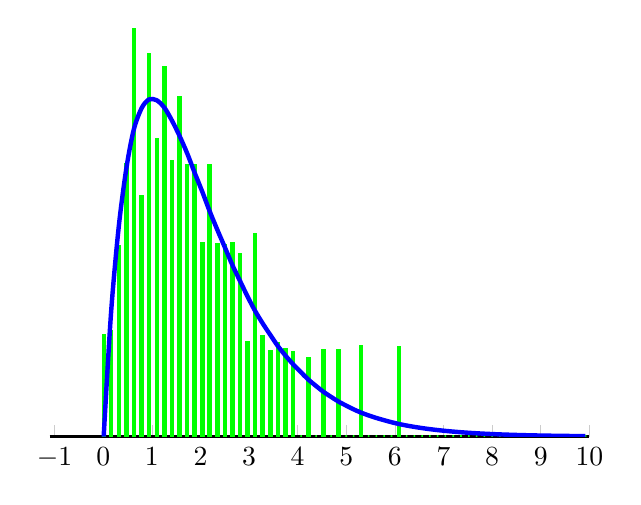
\begin{tikzpicture}
        \begin{axis}[ % title='Fig. 3-5',
            major y tick style = transparent,
            bar width=0.2mm,
            line width=1pt,
            hide y axis,  
            axis x line*=bottom,
            xmin=-1.1, xmax=1e1,% range for the x axis
            xtick={-1, 0, ..., 10},
            ymin=0
            ]
            \addplot[ybar, style={green,fill=green,mark=none}]
            coordinates {(0.01, 161 ) (0.16, 167 ) (0.32, 303 ) (0.48, 433 ) (0.63, 648 ) (0.79, 382 ) (0.94, 607 ) (1.10, 473 ) (1.26, 587 ) (1.41, 438 ) (1.57, 539 ) (1.73, 432 ) (1.88, 431 ) (2.04, 308 ) (2.19, 431 ) (2.35, 306 ) (2.51, 304 ) (2.66, 307 ) (2.82, 290 ) (2.97, 150 ) (3.12, 322 ) (3.28, 159 ) (3.44, 136 ) (3.59, 148 ) (3.75, 138 ) (3.91, 134 ) (4.07, 0   ) (4.22, 124 ) (4.38, 0   ) (4.53, 137 ) (4.69, 0   ) (4.84, 137 ) (5.00, 0   ) (5.15, 0   ) (5.30, 144 ) (5.46, 0   ) (5.62, 0   ) (5.78, 0   ) (5.93, 0   ) (6.08, 142 ) (6.24, 0   ) (6.40, 0   ) (6.56, 0   ) (6.72, 0   ) (6.88, 0   ) (7.04, 0   ) (7.20, 0   ) (7.36, 0   ) (7.52, 0   ) (7.68, 0   ) (7.84, 0   ) (8.00, 0   ) (8.16, 0   ) (8.32, 0   ) (8.48, 0   ) (8.64, 0   ) (8.80, 0   ) (8.96, 0   ) (9.12, 0   ) (9.28, 0   ) (9.44, 0   ) (9.60, 0   ) (9.76, 0   ) (9.92, 0   )};
            \addplot[draw=blue,ultra thick,smooth] 
            coordinates {(0.01, 0.00000) (0.16, 195.12194) (0.32, 333.79328) (0.48, 428.26278) (0.63, 488.41676) (0.79, 522.20624) (0.94, 536.00000) (1.10, 534.87594) (1.26, 522.86130) (1.41, 503.13034) (1.57, 478.16688) (1.73, 449.89758) (1.88, 419.80123) (2.04, 388.99794) (2.19, 358.32200) (2.35, 328.38112) (2.51, 299.60454) (2.66, 272.28193) (2.82, 246.59479) (2.97, 222.64168) (3.12, 200.45844) (3.28, 180.03425) (3.44, 161.32438) (3.59, 144.26024) (3.75, 128.75721) (3.91, 114.72070) (4.07, 102.05085) (4.22, 90.64598) (4.38, 80.40523) (4.53, 71.23046) (4.69, 63.02756) (4.84, 55.70734) (5.00, 49.18608) (5.15, 43.38580) (5.30, 38.23438) (5.46, 33.66547) (5.62, 29.61834) (5.78, 26.03762) (5.93, 22.87308) (6.08, 20.07924) (6.24, 17.61506) (6.40, 15.44363) (6.56, 13.53182) (6.72, 11.84996) (6.88, 10.37153) (7.04, 9.07286) (7.20, 7.93288) (7.36, 6.93286) (7.52, 6.05616) (7.68, 5.28803) (7.84, 4.61540) (8.00, 4.02671) (8.16, 3.51176) (8.32, 3.06154) (8.48, 2.66808) (8.64, 2.32439) (8.80, 2.02430) (8.96, 1.76240) (9.12, 1.53391) (9.28, 1.33464) (9.44, 1.16093) (9.60, 1.00954) (9.76, 0.87766) (9.92, 0.76281)};
            \coordinate (a) at (36,330);
            %\coordinate (b) at (90,600);
                                                                                                                                                \node[rectangle, draw] (b) at (90,600) {$p(x)=xe^{-x}$};
            \draw[->, black] (b) -- (a);
            % \draw[->,blue] (b) -- (a) node [above] {p(x)=xe-x};
        \end{axis}
    \end{tikzpicture}
    \caption{\textit{Random variates from table of 64 from distribution $p(x)=xe^{-x}$}}
    \label{fig:03_05}
\end{figure}

\TallC{With}slightly more elaboration we can arrange for each table to have a unique prng, thus minimizing correlations between tables. Because the resulting data structure is nearly an "object", it is worthwhile to see how this may be done.

To make the prng unique, all that is necessary is to make the seed \textbf{VAR}s unique to a table, and to redefine \textbf{RANDOMIZE} and, \textbf{RANDOM} to know how to get a given table's seeds. We see that \textbf{RANDOM} is invoked only in the runtime code for the structure. This means it has access to the base address, hence the \textbf{VAR}s can be replaced with cells in the table, and the seeds planted there.